\newpage
\section{Vergleich der Emulationsumgebungen}\label{ref:VerglAktSitEmu}
Ein wichtiger Bestandteil in der dynamischen Analyse von Apps ist die Möglichkeit, Applikationen in einer emulierten Umgebung auszuführen. Im Folgenden werden diese Möglichkeiten für die \textit{iOS}, \textit{Windows-Phone} und \textit{Android} getestet.
 
	\subsection{iOS}
	Im Folgenden wurde speziell der in \textit{Xcode} enthaltene, offizielle \textit{iOS}-Simulator in seiner Funktionsweise untersucht.
	
			\subsubsection{Emulation}\label{ref:emulation}
			Die Emulation von \textit{iOS}-Geräten ist derzeit mit der Verwendung von \textit{Xcode} möglich. \textit{Xcode} wiederum ist nur unter \textit{Mac OS X} erhältlich. Da \textit{Max OS X} laut EULA nur auf "`Apple-branded computers"' verwendet werden darf \cite{AppleEULA}, ist die Simulation von \textit{iOS}-Geräten nur unter Apple-Hardware möglich. Nach der Installation über den in \textit{Mac OS X} enthaltenen App-Store kann ein virtualisiertes \textit{iPhone} über die Schritte \textit{XCode} $\rightarrow$ \textit{Open Developer Tools} $\rightarrow$ \textit{Simulator} oder über 
\begin{lstlisting}
/Applications/Xcode.app/Contents/Developer/Applications/Simulator.app
\end{lstlisting}			
gestartet werden.\\
			
		\subsubsection{Debugging}
Als Debugger unter \textit{Mac OS X} hat sich \textit{LLDB} etabliert und stellt das Pendant zu \textit{GDB} unter Linux dar. \textit{LLDB} ist kostenlos verfügbar, Open-Source und steht unter der University of Illinois/NCSA Open Source License\footnote{\url{https://opensource.org/licenses/UoI-NCSA.php}}, welche die Vervielfältigung und Veränderung des Quellcodes unter Hinweis auf \textit{LLVM} erlaubt.\\

\textit{LLDB} sollte auf jedem \textit{Mac OS X} System mit \textit{XCode} automatisch installiert sein und lässt sich im Terminal über das Kommando
\begin{lstlisting}
lldb
\end{lstlisting} aufrufen. Eine Gegenüberstellung von \textit{GDB}-Kommandos zu \textit{LLDB} steht auf der \textit{LLDB}-Webseite\footnote{\url{http://lldb.llvm.org/lldb-gdb.html}} zur Verfügung.\\

 Kompiliert man eine Applikation in \textit{xCode}, wird diese in einem emulierten \textit{iPhone} ge\-star\-tet und direkt ein Fenster \textit{LLDB} geöffnet. Die ausgeführte Applikation ist in \textit{LLDB} automatisch ausgewählt.\\

\begin{figure}[htbp]
	\centering
	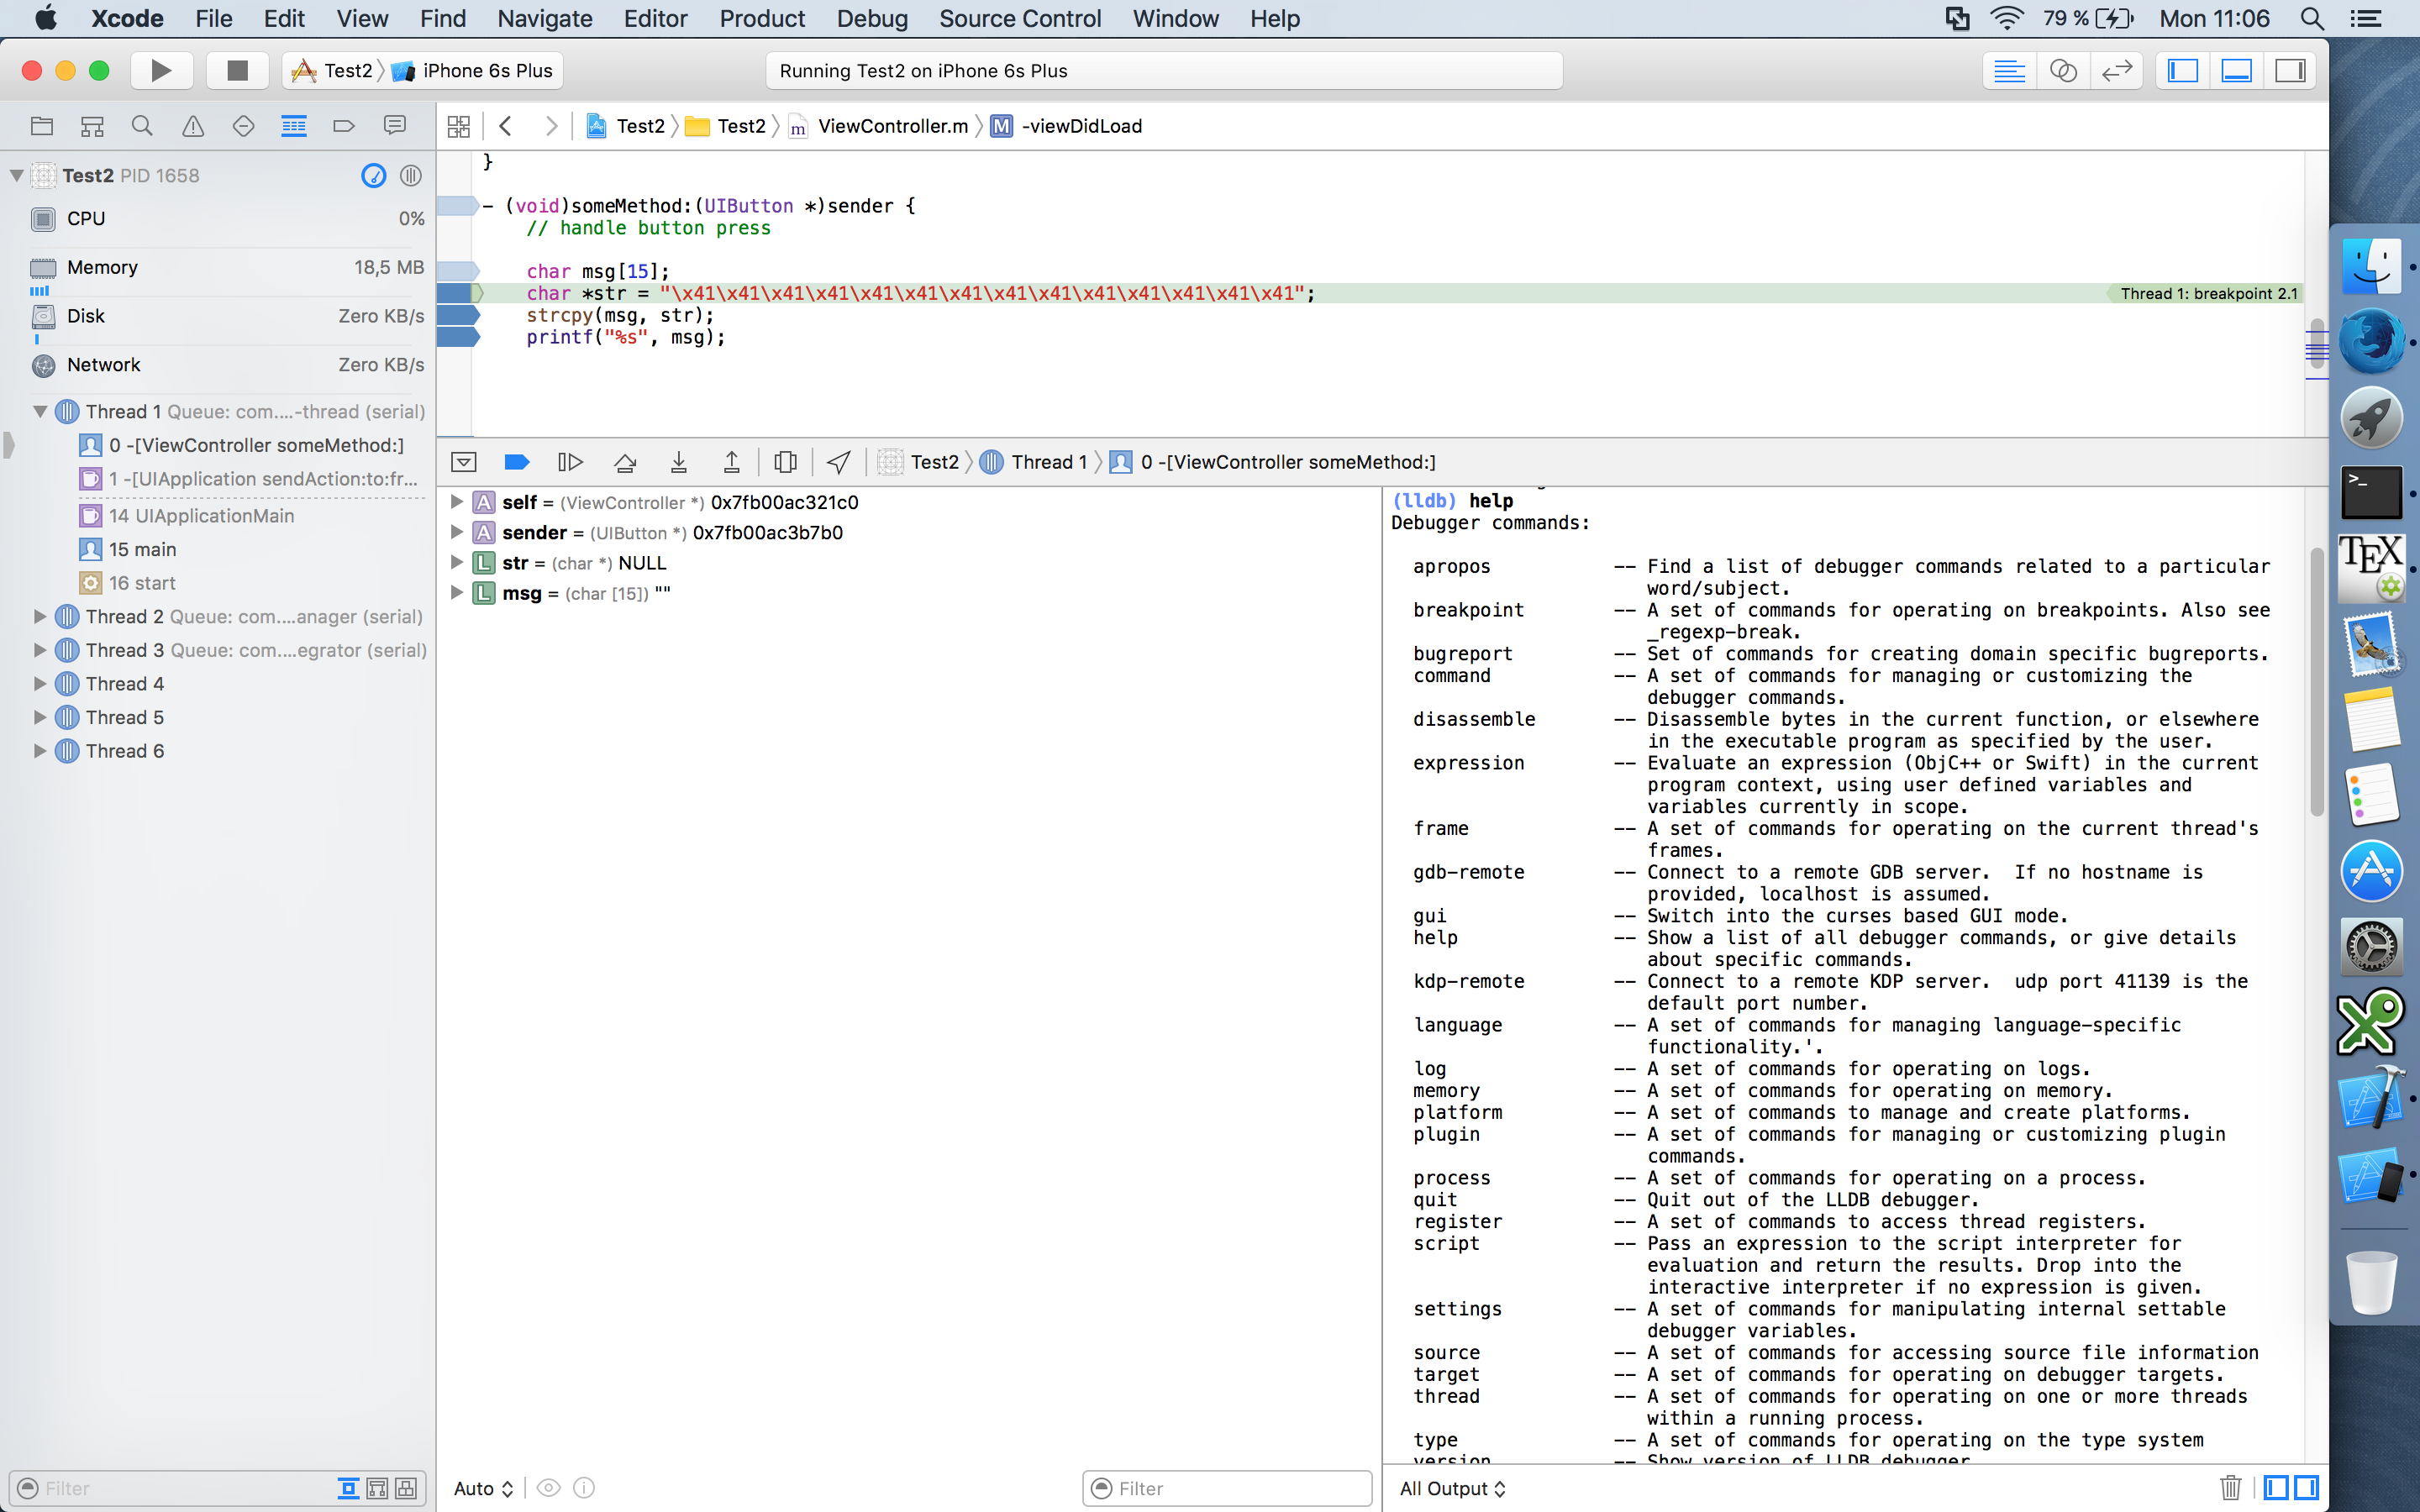
\includegraphics[width=\textwidth]{bilder/pentest_mobile_anwendungen/vergleich_aktuelle_situation/20160627_XCode-LLDB.png}
	\caption{LLDB in XCode}
	\label{fig:LLDBinXCode}
\end{figure}
Ein Ziel dieser Arbeit ist das Automatisieren von Analysen, weshalb das Ausführen der grafischen Oberfläche nicht optimal ist.\\

Leider ist nicht erkennbar, wie \textit{LLDB} und das emulierte \textit{iPhone} eine Verbindung herstellen. Eine Auflistung der offenen Sockets auf dem System legt jedoch nahe, dass auf dem \textit{iPhone} das Programm \textit{debugserver} gestartet wird, welches Remote-Debugging mit \textit{LLDB} erlaubt. Es bleibt herauszufinden, wie die Debugging-Session auf dem simulierten \textit{iPhone} ohne \textit{XCode} hergestellt werden kann.\\

\begin{figure}[htbp]
	\centering
	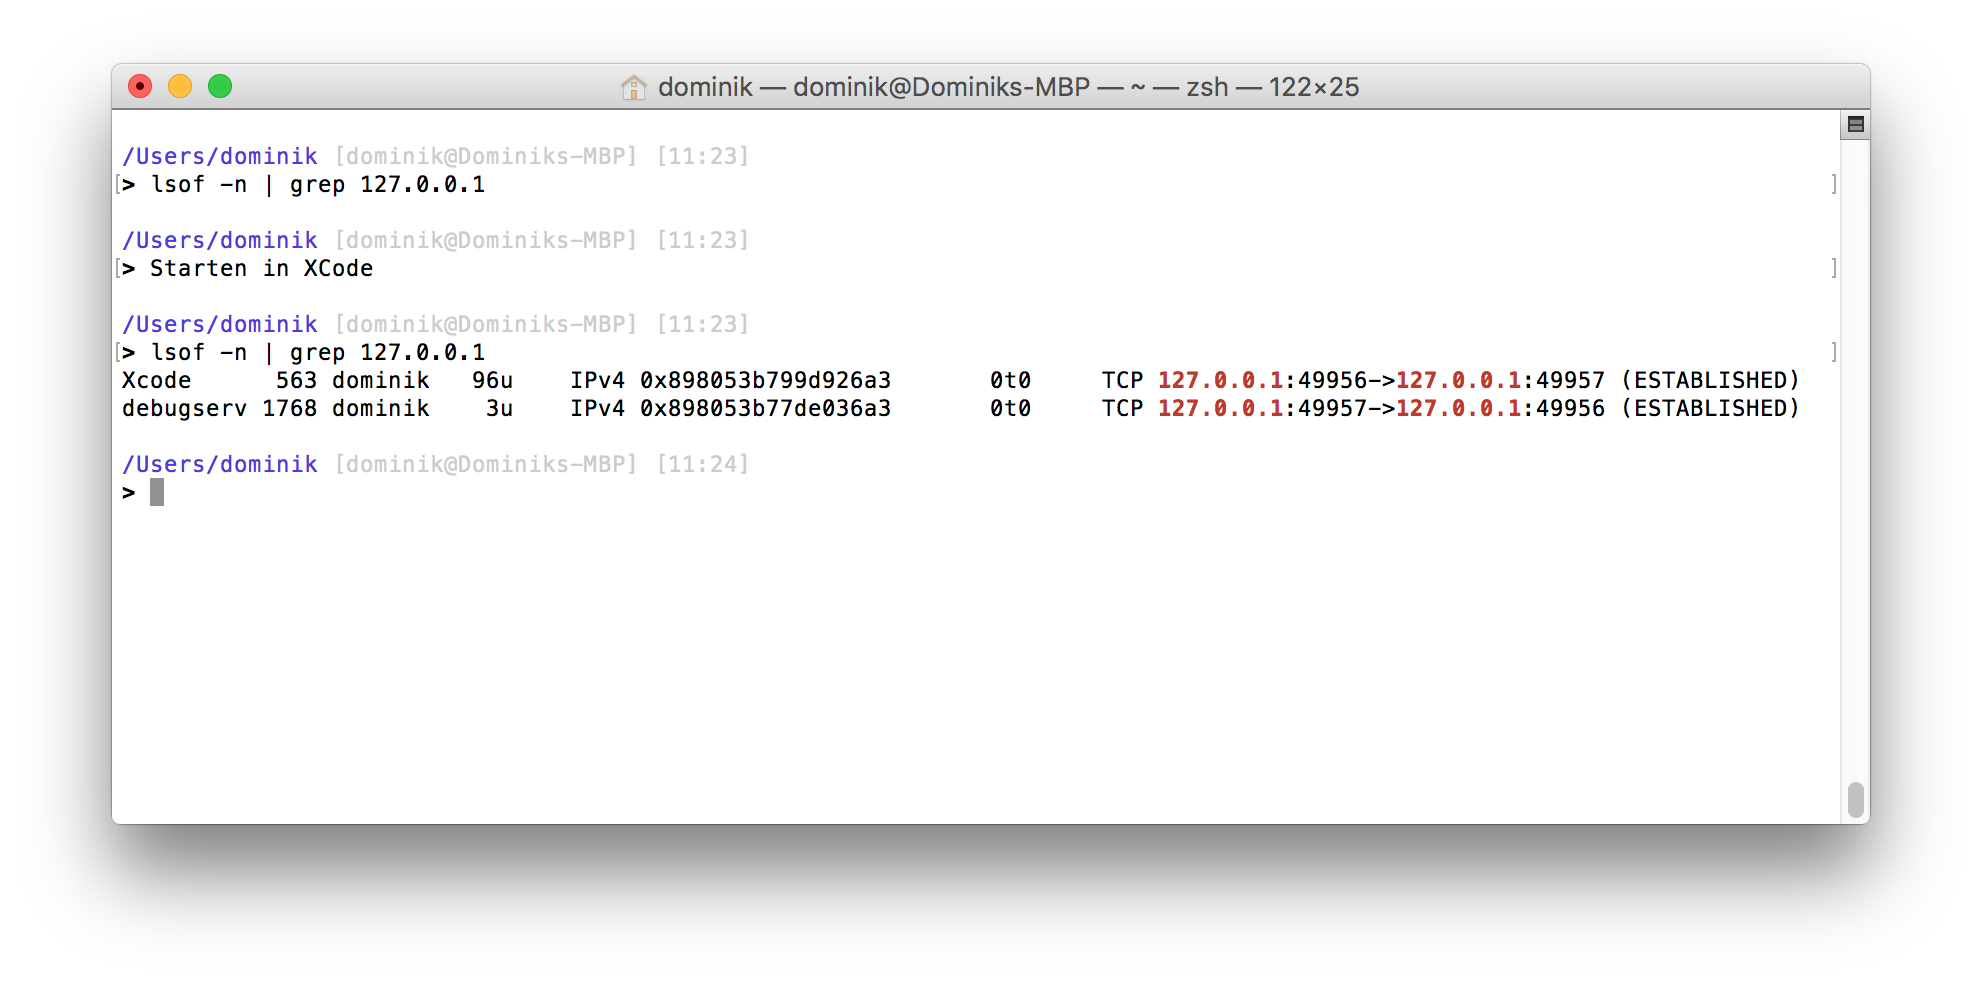
\includegraphics[width=\textwidth]{bilder/pentest_mobile_anwendungen/vergleich_aktuelle_situation/20160627_lsof_XCode_running.png}
	\caption{Vergleich der offenen Pipes vor und nach der Ausführung der Applikation in XCode}
	\label{fig:LSOFLLDB}
\end{figure}

Nach einem Artikel von Apple\footnote{\url{https://developer.apple.com/library/ios/documentation/IDEs/Conceptual/gdb_to_lldb_transition_guide/document/lldb-terminal-workflow-tutorial.html}} ist es möglich, mit \textit{LLDB} eine App auch als "`Standalone Debugger"', also ohne \textit{XCode}, zu verwenden. Dies ist in Abbildung \ref{fig:LLDBStandaloneDebugger} aufgezeigt.\\

\begin{figure}[htbp]
	\centering
	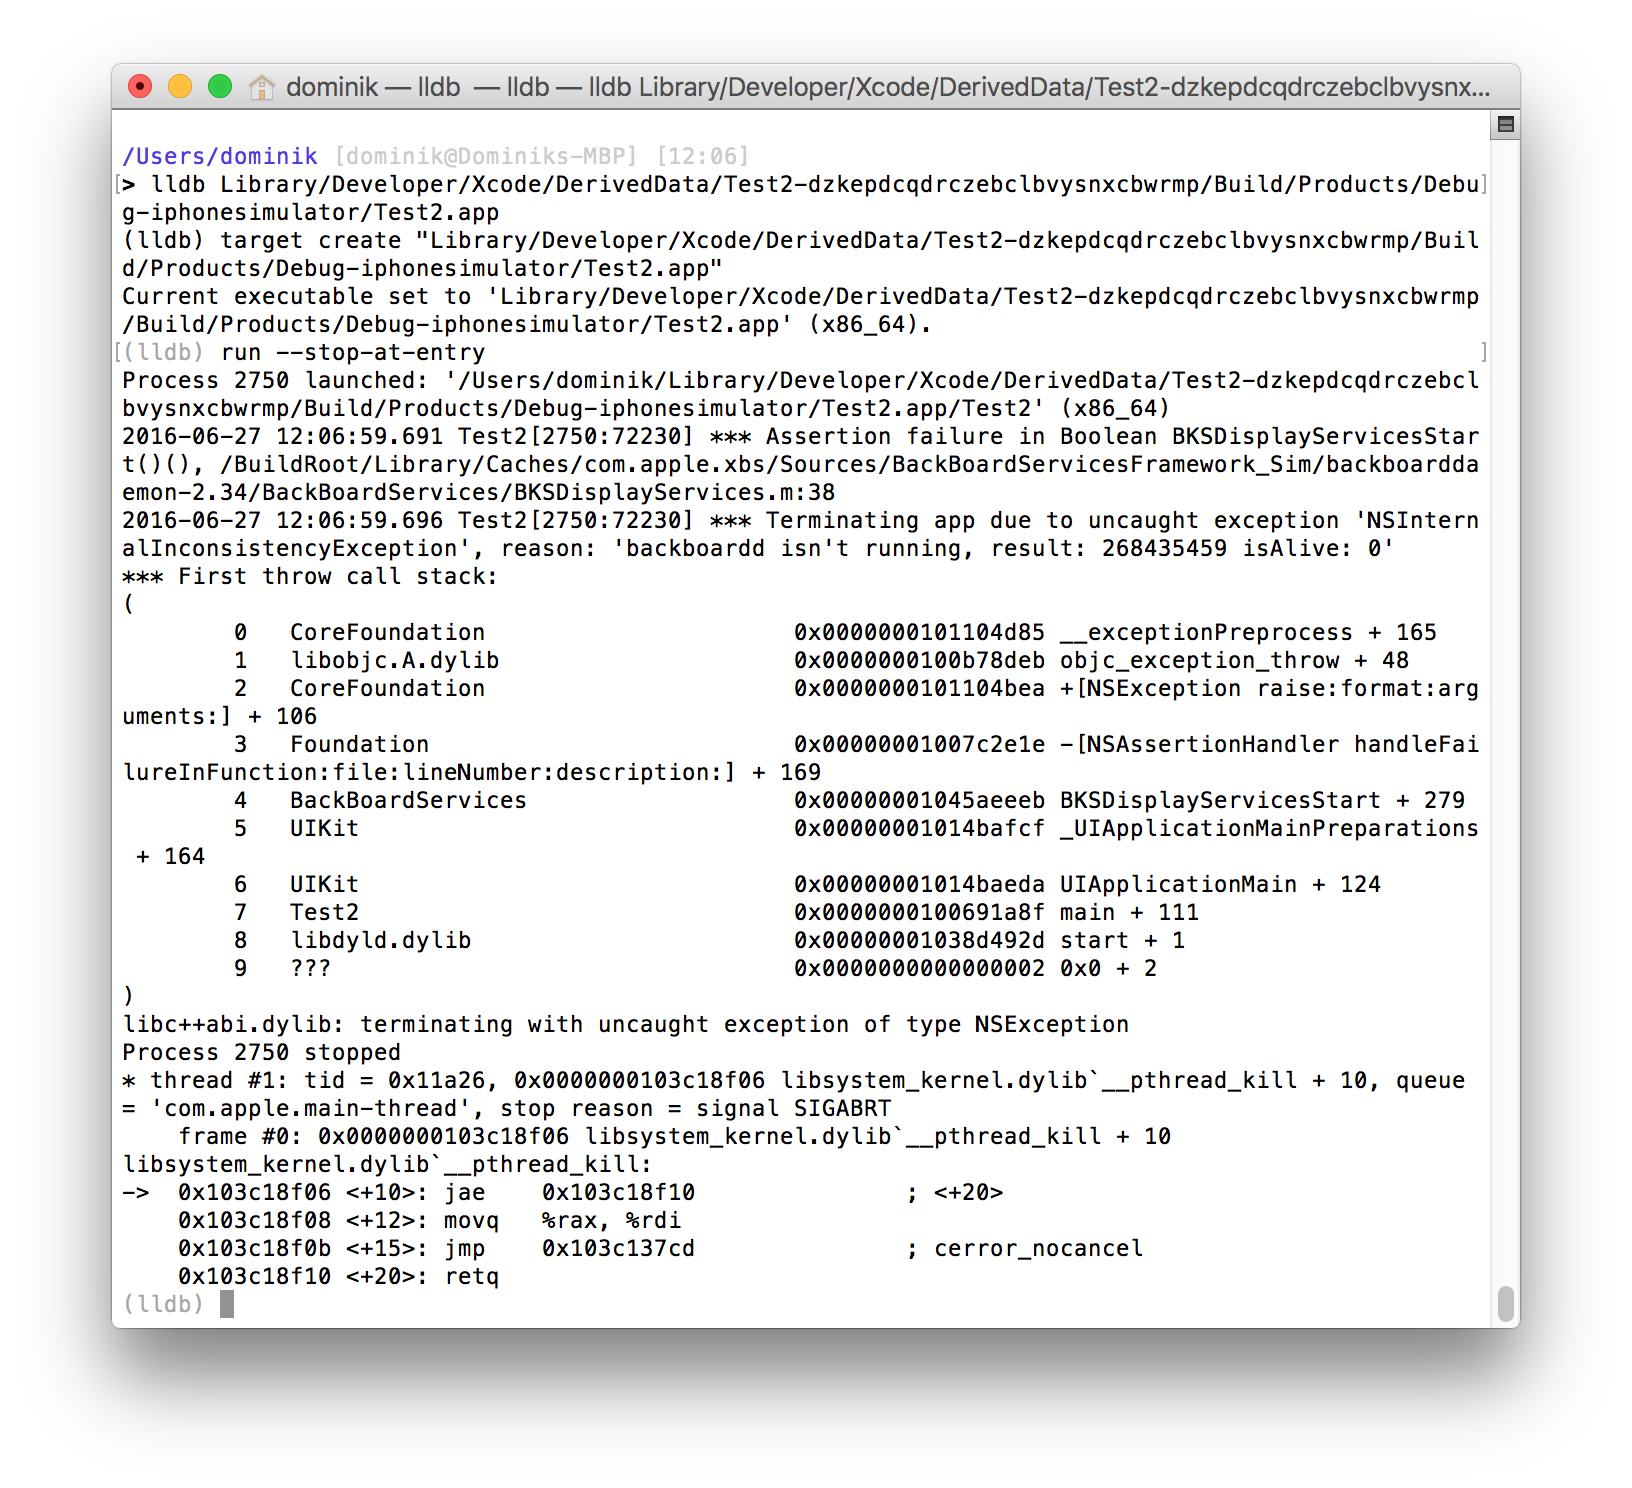
\includegraphics[width=\textwidth]{bilder/pentest_mobile_anwendungen/vergleich_aktuelle_situation/20160627_LLDB-Standalone-Debugger.png}
	\caption{LLDB als Standalone Debugger}
	\label{fig:LLDBStandaloneDebugger}
\end{figure}

Um zu verifizieren, dass die App auf einem simulierten \textit{iPhone} ausgeführt wird, können entweder die geöffneten Prozesse (siehe Abbildung \ref{fig:LLDB-creating-IPhone-VM}) oder die geladenen Bibliotheken der Programme (siehe Abbildung \ref{fig:VergleichLLDBImages}) verglichen werden.\\

\begin{figure}[htbp]
	\centering
	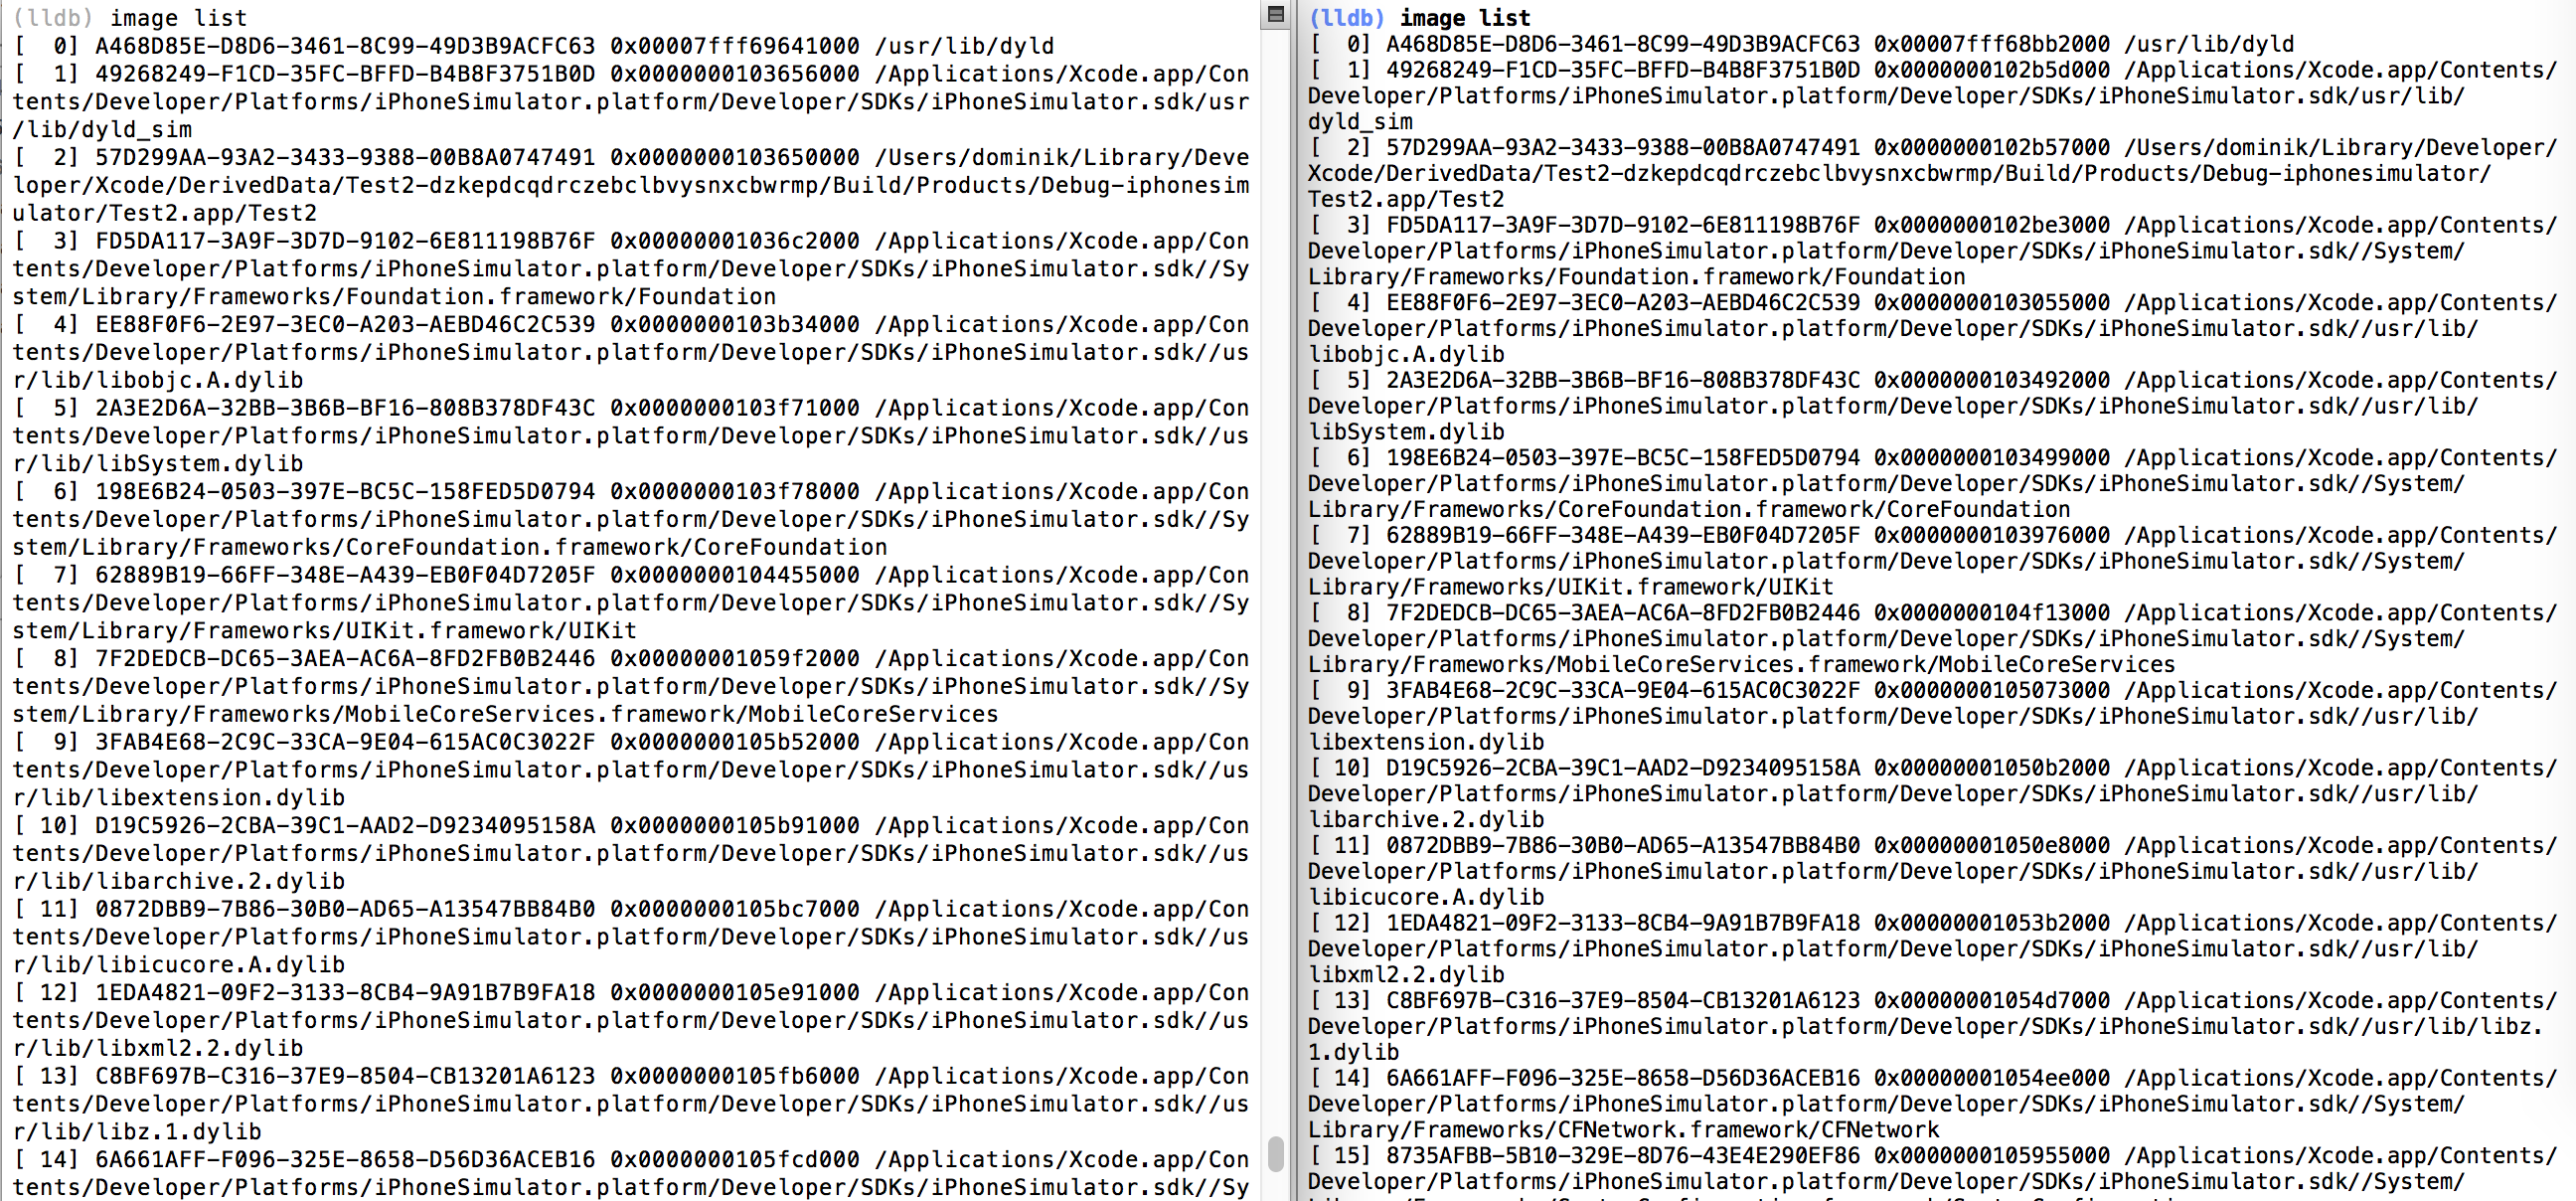
\includegraphics[width=\textwidth]{bilder/pentest_mobile_anwendungen/vergleich_aktuelle_situation/20160627_LLDB-image-list.png}
	\caption{Vergleich der geladenen Bibliotheken}
	\label{fig:VergleichLLDBImages}
\end{figure}

Beide Methoden zeigen, dass die App auf dem simulierten \textit{iPhone} gestartet wird. Bei den Prozessen ist zu beobachten, dass vor Start von \textit{LLDB} nur der Hintergrund-Service ausgeführt wurde. Nach dem Start von \textit{LLDB} dagegen läuft der gesamte Simulator.\\

Auch der Vergleich der geladenen Bibliotheken legt nahe, dass die \textit{LLDB} Standalone und \textit{Xcode} in der gleichen Umgebung ausgeführt werden. Die Adressen im RAM variieren aufgrund von \textit{ASLR} zwar, aber es werden dieselben Bibliotheken verwendet (am Pfad zu erkennen). Dies ist in Grafik \ref{fig:VergleichLLDBImages} dargestellt.

\begin{figure}[htbp]
\lstinputlisting[lastline=16]{logs/20160627_LLDB-creating-IPhone-VM.txt}
\caption{Geöffnete Prozesse vor und während der Ausführung des Emulators}
\label{fig:LLDB-creating-IPhone-VM}
\end{figure}

\subsubsection{Architektur}\label{ref:VergAktSitiOSArch}
Auffällig ist, dass der Simulator nicht die CPU-Architektur eines \textit{iPhones} simuliert, sondern den Code auf dem x86-Prozessor des Mac-Books ausführt. Dies hat den Nachteil, dass Apps aus dem Apple-App-Store, welche für ARM-Prozessoren kompiliert sind, nicht auf dem Simulator ausgeführt werden können. Lediglich Apps, welche für den Simulator in \textit{Xcode} kompiliert wurden, können im Simulator ausgeführt werden. Dadurch ist eine Analyse von Apps ohne Quellcode-Zugriff nicht möglich.

\subsubsection{Sicherheits-Aspekte}
Bei der Analyse von iOS-Apps wurden zwei mögliche Sicherheitslücken testweise in eine App implementiert. Die Lücken sind "`unsichere Funktionen"', welche eine eventuelle \textit{Memory Corruption} mit sich ziehen, und Verbindungen ohne \textit{TLS}-Absicherung.

\pagebreak
\paragraph{Unsichere Funktionen}
Im Gegensatz zu anderen Sprachen sind in \textit{Objective C} für \textit{iOS}-Apps noch Funktionen, welche für \textit{Memory Corruption}-Schwachstellen anfällig sind, vorhanden.\\

So führt folgendes Code-Segment zwar zum Absturz der App, aber könnte bei einer dynamischen Eingabe des zu kopierenden Strings durchaus eine echte Schwachstelle einführen.
\begin{lstlisting}
char msg[15];
char *str = "\x41\x41\x41\x41\x41\x41\x41\x41\x41\x41\x41\x41\x41\x41\x42";
strcpy(msg, str);
\end{lstlisting}

Dies ist auch in der Apple-Online-Dokumentation beschrieben\footnote{\url{https://developer.apple.com/library/content/documentation/Security/Conceptual/SecureCodingGuide/Articles/BufferOverflows.html}}.

\paragraph{Ungesicherte Verbindungen}\label{ref:inseccon}
Ein Sicherheitsfeature ab \textit{iOS 9.0} ist der Umgang von \textit{iOS} mit Netzwerk-Verbindungen. So können ohne erweiterte Konfiguration keine Verbindungen aufgebaut werden, welche nicht dem RFC-Standard 2818  "`HTTP Over TLS"' \footnote{\url{https://tools.ietf.org/html/rfc2818}} folgen. So führt der in Listing \ref{lst:VergliOSTLSAufbau} gezeigte Aufruf einer HTTP-Seite zu der in \ref{lst:VergliOSTLSFehler} gezeigten Fehlermeldung.\\

\begin{figure}[p]
\begin{lstlisting}
NSURL *url = [NSURL URLWithString:@"http://api.ipify.org"];
    NSData *data = [NSData dataWithContentsOfURL:url];
    NSString *ret = [[NSString alloc] initWithData:data encoding:NSUTF8StringEncoding];
    NSLog(@"ret=%@", ret);
\end{lstlisting} 
\caption{Aufbau einer nicht mit TLS gesicherten Verbindung}
\label{lst:VergliOSTLSAufbau}
\end{figure}

\begin{figure}[p]
\begin{lstlisting}
2016-06-28 08:42:56.518 Test2[4789:140270] App Transport Security has blocked a cleartext HTTP (http://) resource load since it is insecure. Temporary exceptions can be configured via your app's Info.plist file.
\end{lstlisting}
\caption{Fehler bei Aufbau einer ungesicherten Verbindung ohne Definition einer Ausnahme}
\label{lst:VergliOSTLSFehler}
\end{figure}

Sollten unsichere Verbindungen benötigt werden, muss ein entsprechender Eintrag in der "`Info.plist"' angelegt werden. Dieser Eintrag muss sehr genau auf die App angepasst werden, da zum Beispiel die Domains festgelegt werden müssen. Ein Eintrag muss laut Apple\cite{AppleNSAppTransportSecurity} den in \ref{lst:VergliOSATSAus} dargestellten Inhalt haben. Eine Überprüfung auf solche Ausnahmen kann dem Abschnitt \ref{ref:WeitMobSFErkennungVonUngesichertenVerbindungen} entnommen werden.

\begin{figure}
\begin{lstlisting}
NSAppTransportSecurity : Dictionary {
    NSAllowsArbitraryLoads : Boolean
    NSAllowsArbitraryLoadsForMedia : Boolean
    NSAllowsArbitraryLoadsInWebContent : Boolean
    NSAllowsLocalNetworking : Boolean
    NSExceptionDomains : Dictionary {
        <domain-name-string> : Dictionary {
            NSIncludesSubdomains : Boolean
            NSExceptionAllowsInsecureHTTPLoads : Boolean
            NSExceptionMinimumTLSVersion : String
            NSExceptionRequiresForwardSecrecy : Boolean   // Default value is YES
            NSRequiresCertificateTransparency : Boolean
        }
    }
}
\end{lstlisting}
\caption{XML-Definition einer Ausnahme der ATS}
\label{lst:VergliOSATSAus}
\end{figure}

		\subsection{Windows-Phone}
		Im Folgenden wurde der in \textit{Visual Studio} enthaltene Emulator für \textit{Windows-Phone}-Apps in seiner Funktionsweise untersucht.
		
			\subsubsection{Emulation}
			Zur Emulation von \textit{Windows-Phones} ist \textit{Visual Studio} notwendig. Im Folgenden wurde \textit{Visual Studio 15} in der \textit{Community Edition}, also einer kostenlosen Version, verwendet.\\
			
			Nach der Installation von \textit{Visual Studio} sollte das Framework für die \textit{Universal Windows Platform} sowie der Emulator installiert werden. Beide können als Optionen bei der Installation gewählt werden. Anschließend kann eine App sowohl im Emulator, als auch lokal auf der Windows-Maschine gestartet werden. Alternativ kann auch ein physikalisches Windows-Gerät für die Ausführung von Apps genutzt werden.
			
			\subsubsection{Debugging}
			Debugging kann direkt über \textit{Visual Studio} durchgeführt werden. Dazu können einfach die jeweiligen Breakpoints im Code gesetzt werden.\\
			
			Eine Möglichkeit zum Debugging außerhalb von \textit{Visual Studio} wurde nicht gefunden, da Microsoft keine öffentlich beschriebene Schnittstelle zur Kommunikation mit Apps innerhalb des Betriebssystems zur Verfügung stellt.
			
			\subsubsection{Unsichere Funktionen}
			Unsichere Funktionen wie "`strcpy"' oder "`memcpy"' sind in den Bibliotheken für \textit{C++}-Apps der \textit{Universal Windows Platform} noch enthalten, können aber ohne erweitere Konfiguration nicht genutzt werden.\\
			
			Um diese Funktionen zu nutzten, muss dem Compiler die Flag 
			\begin{lstlisting}
_CRT_SECURE_NO_WARNINGS			
			\end{lstlisting}
			übergeben werden. Anschließend können auch Funktionen, welche zu \textit{Memory-Corruption} führen können, frei genutzt werden.
			
			\subsubsection{Unsichere Verbindungen}
			Bezüglich unsicherer Verbindungen schreibt die \textit{Universal Windows Platform} nichts vor. So kann über folgenden Aufruf eine Seite ohne TLS aufgerufen werden.
			\begin{lstlisting}
auto uri = ref new Windows::Foundation::Uri("http://api.ipify.org");
webView->Navigate(uri);
			\end{lstlisting}
			
		\subsection{Android}
			\textit{Android} ist ein ursprünglich 2003 von der \textit{Android, Inc.} entwickeltes mobiles Betriebssystem. 2005 wurde es durch Google übernommen und wird seitdem von Google weiterentwickelt. 2015 liegt es in der EU bei einem Marktanteil von $75,6\%$\cite{KatarWorldpanelMobBetrSys}. Aufgrund der Quelloffenheit des Systems wird es von vielen Herstellern auf verschiedensten Plattformen genutzt. Jedoch bringt die weitführende Fragmentierung des Betriebssystems auch Nachteile mit sich. So sind im Februar 2017 nur $1,2 \%$ der Android-Devices auf einer aktuellen Version (Nougat, 7).\cite{StatistaAndroidVersionen}\cite{Drake2014}
			
			\subsubsection{Android-Studio und SDK}
			Das Android-Studio ist eine umfassende IDE. Sie ermöglicht unter anderem das schnelle Entwickeln und Testen von Apps, sowie die Emulation von beliebigen Android-Versionen. Außerdem ist Android Studio kostenlos, Open-Source und für Linux, Mac und Windows erhältlich. Die aktuelle Version kann von der offiziellen Webseite\footnote{\url{http://developer.android.com/sdk/index.html}} heruntergeladen werden. Die Installation unter Linux ist vergleichsweise einfach, da nur ein Archiv über das Kommando 
\begin{lstlisting}
unzip android-studio-ide-143.2739321-linux.zip
\end{lstlisting}
entpackt werden muss. Für alle anderen Betriebssysteme werden entsprechende Installationsroutinen zur Verfügung gestellt. Anschließend kann die IDE über die Datei "`bin/studio.sh"' gestartet werden. Neben dem Android-Studio gibt es noch das Android SDK, welches über die gleiche URL heruntergeladen werde kann. Es enthält wichtige Kommandozeilen-Tools wie \textit{adb}, \textit{fastboot} oder \textit{logcat}, auf welche zum Teil im weiteren Verlauf noch detailliert eingegangen wird.

			%\subsubsection{Compatibility Testing Suite}
			%\cite{Drake2014} Seite 18
			
			\subsubsection{Emulation vs. Hardware}
			Im Gegensatz zum \textit{iOS}-Simulator hat \textit{AVD} die Möglichkeit, CPU wie auch GPU eines Handys zu emulieren. Dabei besteht die Auswahl zwischen verschiedenen Architekturen, wie Intel x86 oder ARM. Zudem gibt es viele andere Möglichkeiten zur Konfiguration der einzelnen Maschinen, wie in Grafik \ref{fig:VergleichAVDConfig} zu sehen ist. Daher hat \textit{Android} den Vorteil, dass gerade tiefgreifende Analysen aufgrund der Emulation der Architektur näher an der echten Hardware sind als bei \textit{iOS}.\cite{Drake2014}
			
			\begin{figure}[htbp]
				\centering
				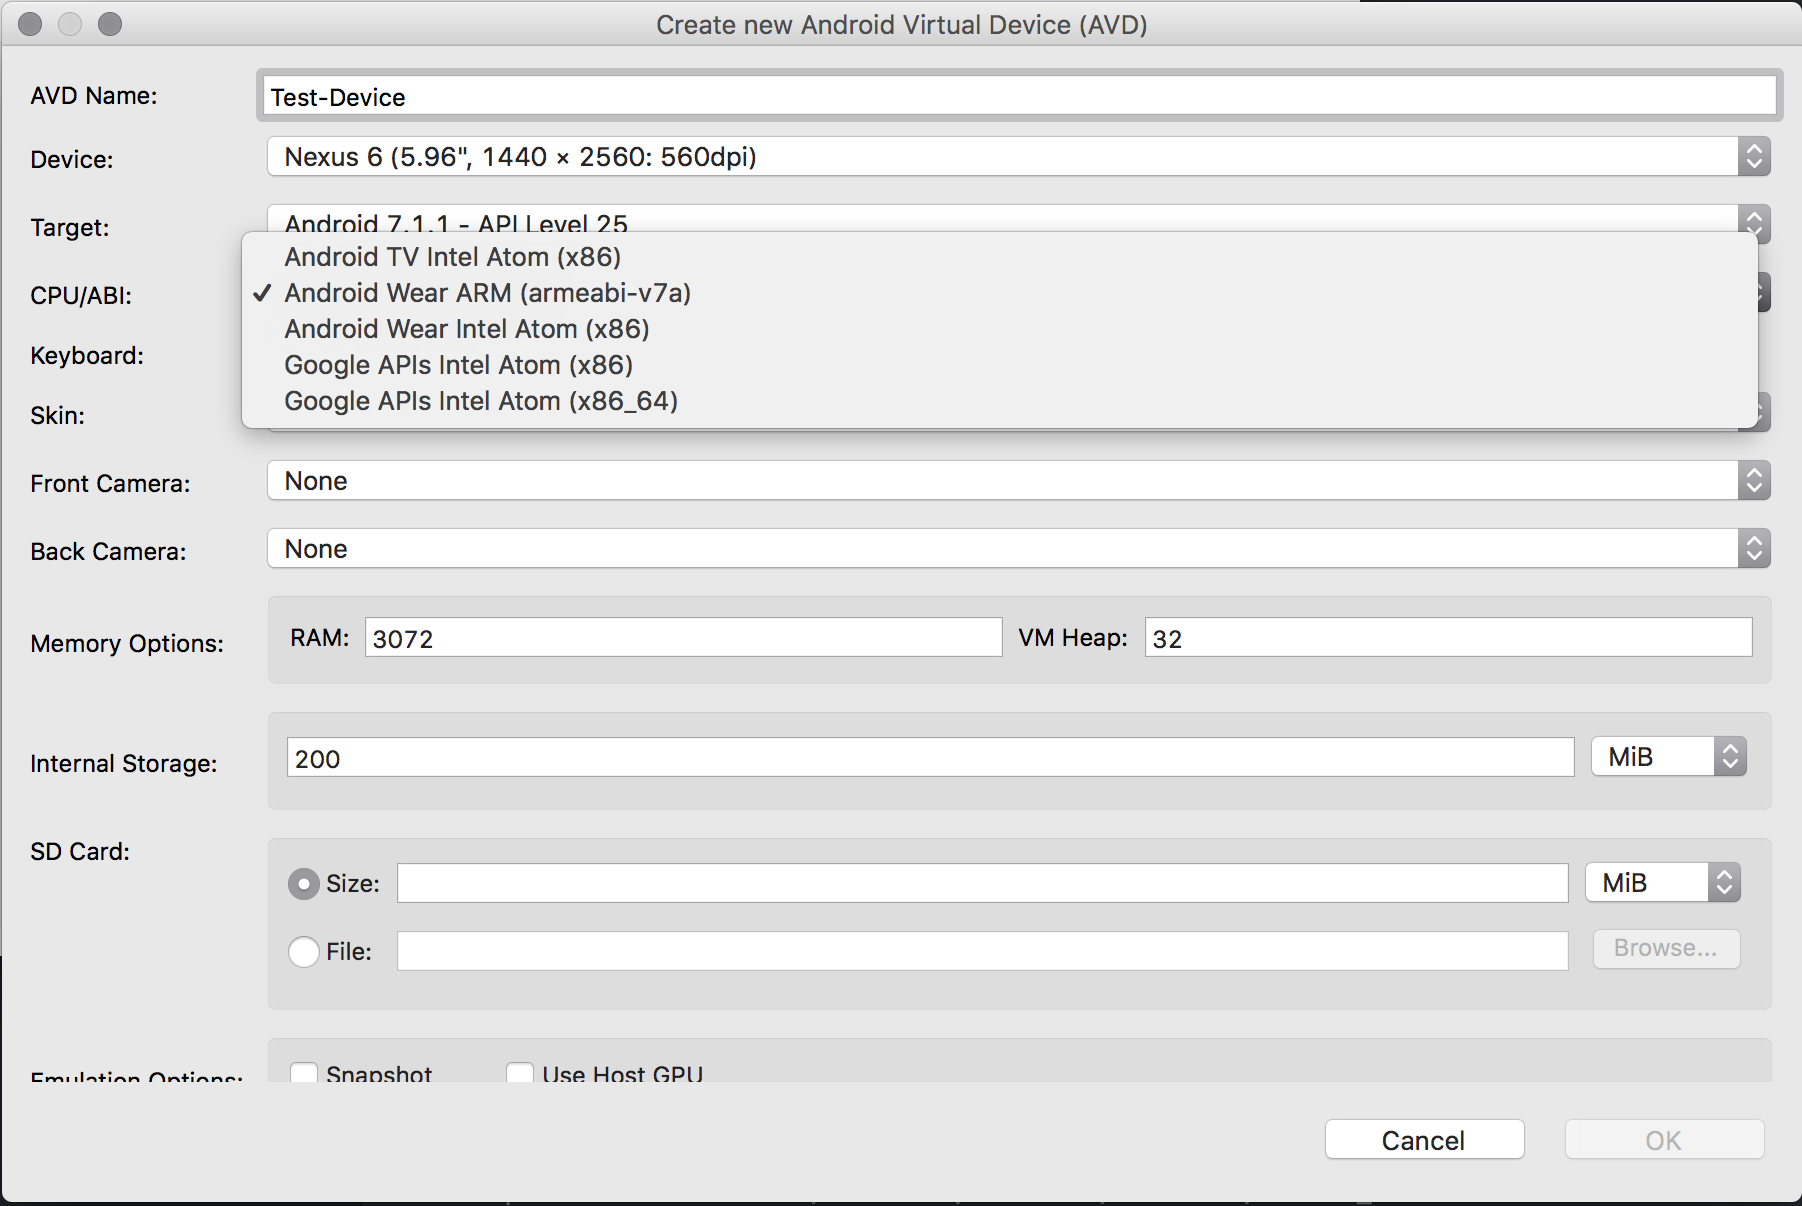
\includegraphics[width=\textwidth]{bilder/pentest_mobile_anwendungen/vergleich_aktuelle_situation/20170215_AVD-Config-Screen.png}
				\caption{Der Konfigurations-Bildschirm des AVD-Managers}
				\label{fig:VergleichAVDConfig}
			\end{figure}
			
			\subsubsection{Debugging}	
			Zum Debugging unter Android kann die \textit{Android Debug Bridge}, kurz \textit{ADB}, genutzt werden. Dabei bietet \textit{ADB} nicht nur die Funktionen für emulierte Geräte, sondern auch für physikalische. Zusätzlich kann für physikalische Geräte sogar Debugging über das Netzwerk durchgeführt werden. Für kabelgebundene oder emulierte Handys können mit dem Aufruf \textit{adb devices} die dem Rechner zur Verfügung stehenden Geräte abgerufen werden. Anschließend können über \textit{adb shell} beliebige Kommandos, inklusive des Aufrufs des internen Debuggers, gegeben werden.\cite{androidDebugBridge}\\
			
			Eine App kann über das Kommando
			\begin{lstlisting}
am start -n <package identifier>/.<activity>
			\end{lstlisting}
			gestartet werden. Dazu muss jedoch die Start-Aktivität der App in Erfahrung gebracht werden. Dies ist über
			\begin{lstlisting}
cmd package resolve-activity --brief <package identifier>
			\end{lstlisting}
			möglich. Um eine App im Debug-Modus zu starten, wird \textit{am} einfach der Parameter \textit{-D} angehängt.
			\begin{lstlisting}
am start -n -D <package identifier>/.<activity>
			\end{lstlisting}
			Allerdings bleibt anzumerken, dass die Debug-Flag für die meisten Apps nicht gesetzt ist. Um dies, insofern notwendig, zu umgehen, muss \textit{am}	als privilegierter User ausgeführt werden. Damit dies möglich ist, muss das Smartphone "`gerooted"', also der Root-Account aktiviert, sein. Alternativ kann auch das APK vom Telefon geladen, die Debug-Flag im \textit{AndroidManifest.xml} ergänzen und wieder am Handy installiert werden.\\
			
			Anschließend kann die App direkt über \textit{jdb}\footnote{\url{https://docs.oracle.com/javase/8/docs/technotes/tools/windows/jdb.html}} oder eine IDE wie IntelliJ debugged werden. Im Detail ist dies zum Beispiel im Blog\footnote{\url{https://blog.netspi.com/attacking-android-applications-with-debuggers/}} von Eric Gruber beschreiben.\\
			
%			Abschließend bleibt zu sagen, dass das Debugging von \textit{Android}-Apps über eine Vielzahl von Wegen und Tools durchgeführt werden kann.
			
			%\subsubsection{Logcat}
			
			%monitor
			%Android Debug Bridge\cite{androidDebugBridge}